\documentclass[twoside]{book}

% Packages required by doxygen
\usepackage{fixltx2e}
\usepackage{calc}
\usepackage{doxygen}
\usepackage[export]{adjustbox} % also loads graphicx
\usepackage{graphicx}
\usepackage[utf8]{inputenc}
\usepackage{makeidx}
\usepackage{multicol}
\usepackage{multirow}
\PassOptionsToPackage{warn}{textcomp}
\usepackage{textcomp}
\usepackage[nointegrals]{wasysym}
\usepackage[table]{xcolor}

% NLS support packages
\usepackage{polski}
\usepackage[T1]{fontenc}

% Font selection
\usepackage[T1]{fontenc}
\usepackage[scaled=.90]{helvet}
\usepackage{courier}
\usepackage{amssymb}
\usepackage{sectsty}
\renewcommand{\familydefault}{\sfdefault}
\allsectionsfont{%
  \fontseries{bc}\selectfont%
  \color{darkgray}%
}
\renewcommand{\DoxyLabelFont}{%
  \fontseries{bc}\selectfont%
  \color{darkgray}%
}
\newcommand{\+}{\discretionary{\mbox{\scriptsize$\hookleftarrow$}}{}{}}

% Page & text layout
\usepackage{geometry}
\geometry{%
  a4paper,%
  top=2.5cm,%
  bottom=2.5cm,%
  left=2.5cm,%
  right=2.5cm%
}
\tolerance=750
\hfuzz=15pt
\hbadness=750
\setlength{\emergencystretch}{15pt}
\setlength{\parindent}{0cm}
\setlength{\parskip}{3ex plus 2ex minus 2ex}
\makeatletter
\renewcommand{\paragraph}{%
  \@startsection{paragraph}{4}{0ex}{-1.0ex}{1.0ex}{%
    \normalfont\normalsize\bfseries\SS@parafont%
  }%
}
\renewcommand{\subparagraph}{%
  \@startsection{subparagraph}{5}{0ex}{-1.0ex}{1.0ex}{%
    \normalfont\normalsize\bfseries\SS@subparafont%
  }%
}
\makeatother

% Headers & footers
\usepackage{fancyhdr}
\pagestyle{fancyplain}
\fancyhead[LE]{\fancyplain{}{\bfseries\thepage}}
\fancyhead[CE]{\fancyplain{}{}}
\fancyhead[RE]{\fancyplain{}{\bfseries\leftmark}}
\fancyhead[LO]{\fancyplain{}{\bfseries\rightmark}}
\fancyhead[CO]{\fancyplain{}{}}
\fancyhead[RO]{\fancyplain{}{\bfseries\thepage}}
\fancyfoot[LE]{\fancyplain{}{}}
\fancyfoot[CE]{\fancyplain{}{}}
\fancyfoot[RE]{\fancyplain{}{\bfseries\scriptsize Wygenerowano przez Doxygen }}
\fancyfoot[LO]{\fancyplain{}{\bfseries\scriptsize Wygenerowano przez Doxygen }}
\fancyfoot[CO]{\fancyplain{}{}}
\fancyfoot[RO]{\fancyplain{}{}}
\renewcommand{\footrulewidth}{0.4pt}
\renewcommand{\chaptermark}[1]{%
  \markboth{#1}{}%
}
\renewcommand{\sectionmark}[1]{%
  \markright{\thesection\ #1}%
}

% Indices & bibliography
\usepackage{natbib}
\usepackage[titles]{tocloft}
\setcounter{tocdepth}{3}
\setcounter{secnumdepth}{5}
\makeindex

% Hyperlinks (required, but should be loaded last)
\usepackage{ifpdf}
\ifpdf
  \usepackage[pdftex,pagebackref=true]{hyperref}
\else
  \usepackage[ps2pdf,pagebackref=true]{hyperref}
\fi
\hypersetup{%
  colorlinks=true,%
  linkcolor=blue,%
  citecolor=blue,%
  unicode%
}

% Custom commands
\newcommand{\clearemptydoublepage}{%
  \newpage{\pagestyle{empty}\cleardoublepage}%
}

\usepackage{caption}
\captionsetup{labelsep=space,justification=centering,font={bf},singlelinecheck=off,skip=4pt,position=top}

%===== C O N T E N T S =====

\begin{document}

% Titlepage & ToC
\hypersetup{pageanchor=false,
             bookmarksnumbered=true,
             pdfencoding=unicode
            }
\pagenumbering{alph}
\begin{titlepage}
\vspace*{7cm}
\begin{center}%
{\Large Suplement\+SelectorC\# }\\
\vspace*{1cm}
{\large Wygenerowano przez Doxygen 1.8.13}\\
\end{center}
\end{titlepage}
\clearemptydoublepage
\pagenumbering{roman}
\tableofcontents
\clearemptydoublepage
\pagenumbering{arabic}
\hypersetup{pageanchor=true}

%--- Begin generated contents ---
\chapter{Indeks przestrzeni nazw}
\section{Pakiety}
Oto lista pakietów wraz z krótkim opisem (o ile jest dostępny)\+:\begin{DoxyCompactList}
\item\contentsline{section}{\hyperlink{namespace_wpf_basics}{Wpf\+Basics} }{\pageref{namespace_wpf_basics}}{}
\item\contentsline{section}{\hyperlink{namespace_wpf_basics_1_1_data}{Wpf\+Basics.\+Data} }{\pageref{namespace_wpf_basics_1_1_data}}{}
\end{DoxyCompactList}

\chapter{Indeks hierarchiczny}
\section{Hierarchia klas}
Ta lista dziedziczenia posortowana jest z grubsza, choć nie całkowicie, alfabetycznie\+:\begin{DoxyCompactList}
\item \contentsline{section}{Wpf\+Basics.\+Data.\+Data\+Loader}{\pageref{class_wpf_basics_1_1_data_1_1_data_loader}}{}
\item \contentsline{section}{Wpf\+Basics.\+Data.\+I\+Health\+Problems\+Rest\+Client}{\pageref{interface_wpf_basics_1_1_data_1_1_i_health_problems_rest_client}}{}
\begin{DoxyCompactList}
\item \contentsline{section}{Wpf\+Basics.\+Data.\+Health\+Problems\+Rest\+Client}{\pageref{class_wpf_basics_1_1_data_1_1_health_problems_rest_client}}{}
\end{DoxyCompactList}
\item I\+Notify\+Property\+Changed\begin{DoxyCompactList}
\item \contentsline{section}{Wpf\+Basics.\+Data.\+Health\+Problem}{\pageref{class_wpf_basics_1_1_data_1_1_health_problem}}{}
\item \contentsline{section}{Wpf\+Basics.\+Data.\+Selected\+Item}{\pageref{class_wpf_basics_1_1_data_1_1_selected_item}}{}
\item \contentsline{section}{Wpf\+Basics.\+Data.\+Suplement}{\pageref{class_wpf_basics_1_1_data_1_1_suplement}}{}
\end{DoxyCompactList}
\item Window\begin{DoxyCompactList}
\item \contentsline{section}{Wpf\+Basics.\+Main\+Window}{\pageref{class_wpf_basics_1_1_main_window}}{}
\end{DoxyCompactList}
\end{DoxyCompactList}

\chapter{Indeks klas}
\section{Lista klas}
Tutaj znajdują się klasy, struktury, unie i interfejsy wraz z ich krótkimi opisami\+:\begin{DoxyCompactList}
\item\contentsline{section}{\hyperlink{class_wpf_basics_1_1_data_1_1_data_loader}{Wpf\+Basics.\+Data.\+Data\+Loader} \\*Klasa \hyperlink{class_wpf_basics_1_1_data_1_1_data_loader}{Data\+Loader}, pobieranie danych }{\pageref{class_wpf_basics_1_1_data_1_1_data_loader}}{}
\item\contentsline{section}{\hyperlink{class_wpf_basics_1_1_data_1_1_health_problem}{Wpf\+Basics.\+Data.\+Health\+Problem} \\*Klasa \hyperlink{class_wpf_basics_1_1_data_1_1_health_problem}{Health\+Problem}, deklaracja składowych }{\pageref{class_wpf_basics_1_1_data_1_1_health_problem}}{}
\item\contentsline{section}{\hyperlink{class_wpf_basics_1_1_data_1_1_health_problems_rest_client}{Wpf\+Basics.\+Data.\+Health\+Problems\+Rest\+Client} \\*Klasa Health\+Problem\+Rest\+Client, utworzenie Resta, połączenie z serwerem Javy }{\pageref{class_wpf_basics_1_1_data_1_1_health_problems_rest_client}}{}
\item\contentsline{section}{\hyperlink{interface_wpf_basics_1_1_data_1_1_i_health_problems_rest_client}{Wpf\+Basics.\+Data.\+I\+Health\+Problems\+Rest\+Client} \\*Klasa I\+Health\+Problem\+Rest\+Client, Interfejs utworzony na potrzeby testów jednostkowych }{\pageref{interface_wpf_basics_1_1_data_1_1_i_health_problems_rest_client}}{}
\item\contentsline{section}{\hyperlink{class_wpf_basics_1_1_main_window}{Wpf\+Basics.\+Main\+Window} \\*Logika interakcji dla klasy Main\+Window.\+xaml }{\pageref{class_wpf_basics_1_1_main_window}}{}
\item\contentsline{section}{\hyperlink{class_wpf_basics_1_1_data_1_1_selected_item}{Wpf\+Basics.\+Data.\+Selected\+Item} \\*Klasa \hyperlink{class_wpf_basics_1_1_data_1_1_selected_item}{Selected\+Item}, obsługa zdarzeń }{\pageref{class_wpf_basics_1_1_data_1_1_selected_item}}{}
\item\contentsline{section}{\hyperlink{class_wpf_basics_1_1_data_1_1_suplement}{Wpf\+Basics.\+Data.\+Suplement} \\*Klasa \hyperlink{class_wpf_basics_1_1_data_1_1_suplement}{Suplement}, deklaracja składowych }{\pageref{class_wpf_basics_1_1_data_1_1_suplement}}{}
\end{DoxyCompactList}

\chapter{Dokumentacja przestrzeni nazw}
\hypertarget{namespace_wpf_basics}{}\section{Dokumentacja przestrzeni nazw Wpf\+Basics}
\label{namespace_wpf_basics}\index{Wpf\+Basics@{Wpf\+Basics}}
\subsection*{Przestrzenie nazw}
\begin{DoxyCompactItemize}
\end{DoxyCompactItemize}
\subsection*{Komponenty}
\begin{DoxyCompactItemize}
\item 
class \hyperlink{class_wpf_basics_1_1_main_window}{Main\+Window}
\begin{DoxyCompactList}\small\item\em Logika interakcji dla klasy Main\+Window.\+xaml \end{DoxyCompactList}\end{DoxyCompactItemize}

\hypertarget{namespace_wpf_basics_1_1_data}{}\section{Dokumentacja przestrzeni nazw Wpf\+Basics.\+Data}
\label{namespace_wpf_basics_1_1_data}\index{Wpf\+Basics.\+Data@{Wpf\+Basics.\+Data}}
\subsection*{Komponenty}
\begin{DoxyCompactItemize}
\item 
class \hyperlink{class_wpf_basics_1_1_data_1_1_data_loader}{Data\+Loader}
\begin{DoxyCompactList}\small\item\em Klasa \hyperlink{class_wpf_basics_1_1_data_1_1_data_loader}{Data\+Loader}, pobieranie danych. \end{DoxyCompactList}\item 
class \hyperlink{class_wpf_basics_1_1_data_1_1_health_problem}{Health\+Problem}
\begin{DoxyCompactList}\small\item\em Klasa \hyperlink{class_wpf_basics_1_1_data_1_1_health_problem}{Health\+Problem}, deklaracja składowych. \end{DoxyCompactList}\item 
class \hyperlink{class_wpf_basics_1_1_data_1_1_health_problems_rest_client}{Health\+Problems\+Rest\+Client}
\begin{DoxyCompactList}\small\item\em Klasa Health\+Problem\+Rest\+Client, utworzenie Resta, połączenie z serwerem Javy. \end{DoxyCompactList}\item 
interface \hyperlink{interface_wpf_basics_1_1_data_1_1_i_health_problems_rest_client}{I\+Health\+Problems\+Rest\+Client}
\begin{DoxyCompactList}\small\item\em Klasa I\+Health\+Problem\+Rest\+Client, Interfejs utworzony na potrzeby testów jednostkowych. \end{DoxyCompactList}\item 
class \hyperlink{class_wpf_basics_1_1_data_1_1_selected_item}{Selected\+Item}
\begin{DoxyCompactList}\small\item\em Klasa \hyperlink{class_wpf_basics_1_1_data_1_1_selected_item}{Selected\+Item}, obsługa zdarzeń \end{DoxyCompactList}\item 
class \hyperlink{class_wpf_basics_1_1_data_1_1_suplement}{Suplement}
\begin{DoxyCompactList}\small\item\em Klasa \hyperlink{class_wpf_basics_1_1_data_1_1_suplement}{Suplement}, deklaracja składowych. \end{DoxyCompactList}\end{DoxyCompactItemize}

\chapter{Dokumentacja klas}
\hypertarget{class_wpf_basics_1_1_data_1_1_data_loader}{}\section{Dokumentacja klasy Wpf\+Basics.\+Data.\+Data\+Loader}
\label{class_wpf_basics_1_1_data_1_1_data_loader}\index{Wpf\+Basics.\+Data.\+Data\+Loader@{Wpf\+Basics.\+Data.\+Data\+Loader}}


Klasa \hyperlink{class_wpf_basics_1_1_data_1_1_data_loader}{Data\+Loader}, pobieranie danych.  


\subsection*{Metody publiczne}
\begin{DoxyCompactItemize}
\item 
\mbox{\Hypertarget{class_wpf_basics_1_1_data_1_1_data_loader_a59982b631a3e5f3cb376a4f539a6ac0c}\label{class_wpf_basics_1_1_data_1_1_data_loader_a59982b631a3e5f3cb376a4f539a6ac0c}} 
{\bfseries Data\+Loader} (\hyperlink{interface_wpf_basics_1_1_data_1_1_i_health_problems_rest_client}{I\+Health\+Problems\+Rest\+Client} health\+Problems\+Rest\+Client)
\item 
\hyperlink{class_wpf_basics_1_1_data_1_1_selected_item}{Selected\+Item} \hyperlink{class_wpf_basics_1_1_data_1_1_data_loader_aa993e4aee4e7404e6458e6221174b4db}{Load\+Data} ()
\begin{DoxyCompactList}\small\item\em metoda Load\+Data -\/ wczytanie danych \end{DoxyCompactList}\end{DoxyCompactItemize}


\subsection{Opis szczegółowy}
Klasa \hyperlink{class_wpf_basics_1_1_data_1_1_data_loader}{Data\+Loader}, pobieranie danych. 

ustawienie obiektu dla Bindingu, utworzenie data\+Loader 

\subsection{Dokumentacja funkcji składowych}
\mbox{\Hypertarget{class_wpf_basics_1_1_data_1_1_data_loader_aa993e4aee4e7404e6458e6221174b4db}\label{class_wpf_basics_1_1_data_1_1_data_loader_aa993e4aee4e7404e6458e6221174b4db}} 
\index{Wpf\+Basics\+::\+Data\+::\+Data\+Loader@{Wpf\+Basics\+::\+Data\+::\+Data\+Loader}!Load\+Data@{Load\+Data}}
\index{Load\+Data@{Load\+Data}!Wpf\+Basics\+::\+Data\+::\+Data\+Loader@{Wpf\+Basics\+::\+Data\+::\+Data\+Loader}}
\subsubsection{\texorpdfstring{Load\+Data()}{LoadData()}}
{\footnotesize\ttfamily \hyperlink{class_wpf_basics_1_1_data_1_1_selected_item}{Selected\+Item} Wpf\+Basics.\+Data.\+Data\+Loader.\+Load\+Data (\begin{DoxyParamCaption}{ }\end{DoxyParamCaption})}



metoda Load\+Data -\/ wczytanie danych 

Konwersja J\+S\+ON\textquotesingle{}a na obiekt z C\#, ustawienie danych dla UI 

Dokumentacja dla tej klasy została wygenerowana z pliku\+:\begin{DoxyCompactItemize}
\item 
C\+:/\+Users/\+Maria/\+Desktop/\+Suplement\+Selector\+C/Data\+Loader.\+cs\end{DoxyCompactItemize}

\hypertarget{class_wpf_basics_1_1_data_1_1_health_problem}{}\section{Dokumentacja klasy Wpf\+Basics.\+Data.\+Health\+Problem}
\label{class_wpf_basics_1_1_data_1_1_health_problem}\index{Wpf\+Basics.\+Data.\+Health\+Problem@{Wpf\+Basics.\+Data.\+Health\+Problem}}


Klasa \hyperlink{class_wpf_basics_1_1_data_1_1_health_problem}{Health\+Problem}, deklaracja składowych.  


Diagram dziedziczenia dla Wpf\+Basics.\+Data.\+Health\+Problem\begin{figure}[H]
\begin{center}
\leavevmode
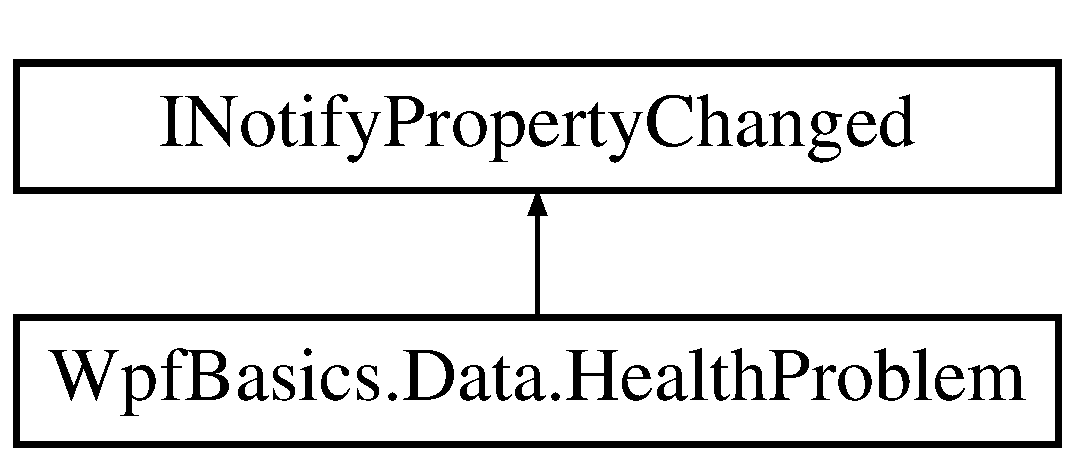
\includegraphics[height=2.000000cm]{class_wpf_basics_1_1_data_1_1_health_problem}
\end{center}
\end{figure}
\subsection*{Metody publiczne}
\begin{DoxyCompactItemize}
\item 
override string \hyperlink{class_wpf_basics_1_1_data_1_1_health_problem_af0aa53844c1f023b9653b789a6a5636a}{To\+String} ()
\end{DoxyCompactItemize}
\subsection*{Właściwości}
\begin{DoxyCompactItemize}
\item 
String \hyperlink{class_wpf_basics_1_1_data_1_1_health_problem_af5f105578193c56e096803bdc26eac8f}{Name}\hspace{0.3cm}{\ttfamily  \mbox{[}get, set\mbox{]}}
\item 
String \hyperlink{class_wpf_basics_1_1_data_1_1_health_problem_a388d29276908852b554ff5afac509640}{Description}\hspace{0.3cm}{\ttfamily  \mbox{[}get, set\mbox{]}}
\item 
String \hyperlink{class_wpf_basics_1_1_data_1_1_health_problem_a49960c2c156d8143d6b07e21467e8794}{Cause}\hspace{0.3cm}{\ttfamily  \mbox{[}get, set\mbox{]}}
\item 
List$<$ \hyperlink{class_wpf_basics_1_1_data_1_1_suplement}{Suplement} $>$ \hyperlink{class_wpf_basics_1_1_data_1_1_health_problem_af68e23b91811f240ec3c6e53dd5ed680}{Suplements}\hspace{0.3cm}{\ttfamily  \mbox{[}get, set\mbox{]}}
\end{DoxyCompactItemize}
\subsection*{Zdarzenia}
\begin{DoxyCompactItemize}
\item 
\mbox{\Hypertarget{class_wpf_basics_1_1_data_1_1_health_problem_af2a436bfdd3a09d529980c52dfaa9f7a}\label{class_wpf_basics_1_1_data_1_1_health_problem_af2a436bfdd3a09d529980c52dfaa9f7a}} 
Property\+Changed\+Event\+Handler {\bfseries Property\+Changed}
\end{DoxyCompactItemize}


\subsection{Opis szczegółowy}
Klasa \hyperlink{class_wpf_basics_1_1_data_1_1_health_problem}{Health\+Problem}, deklaracja składowych. 

gettey i settery 

\subsection{Dokumentacja funkcji składowych}
\mbox{\Hypertarget{class_wpf_basics_1_1_data_1_1_health_problem_af0aa53844c1f023b9653b789a6a5636a}\label{class_wpf_basics_1_1_data_1_1_health_problem_af0aa53844c1f023b9653b789a6a5636a}} 
\index{Wpf\+Basics\+::\+Data\+::\+Health\+Problem@{Wpf\+Basics\+::\+Data\+::\+Health\+Problem}!To\+String@{To\+String}}
\index{To\+String@{To\+String}!Wpf\+Basics\+::\+Data\+::\+Health\+Problem@{Wpf\+Basics\+::\+Data\+::\+Health\+Problem}}
\subsubsection{\texorpdfstring{To\+String()}{ToString()}}
{\footnotesize\ttfamily override string Wpf\+Basics.\+Data.\+Health\+Problem.\+To\+String (\begin{DoxyParamCaption}{ }\end{DoxyParamCaption})}

$<$ zwraca nazwe problemu 

\subsection{Dokumentacja właściwości}
\mbox{\Hypertarget{class_wpf_basics_1_1_data_1_1_health_problem_a49960c2c156d8143d6b07e21467e8794}\label{class_wpf_basics_1_1_data_1_1_health_problem_a49960c2c156d8143d6b07e21467e8794}} 
\index{Wpf\+Basics\+::\+Data\+::\+Health\+Problem@{Wpf\+Basics\+::\+Data\+::\+Health\+Problem}!Cause@{Cause}}
\index{Cause@{Cause}!Wpf\+Basics\+::\+Data\+::\+Health\+Problem@{Wpf\+Basics\+::\+Data\+::\+Health\+Problem}}
\subsubsection{\texorpdfstring{Cause}{Cause}}
{\footnotesize\ttfamily String Wpf\+Basics.\+Data.\+Health\+Problem.\+Cause\hspace{0.3cm}{\ttfamily [get]}, {\ttfamily [set]}}

$<$ pobieranie i ustawianie wartości składowej przyczyny problemu \mbox{\Hypertarget{class_wpf_basics_1_1_data_1_1_health_problem_a388d29276908852b554ff5afac509640}\label{class_wpf_basics_1_1_data_1_1_health_problem_a388d29276908852b554ff5afac509640}} 
\index{Wpf\+Basics\+::\+Data\+::\+Health\+Problem@{Wpf\+Basics\+::\+Data\+::\+Health\+Problem}!Description@{Description}}
\index{Description@{Description}!Wpf\+Basics\+::\+Data\+::\+Health\+Problem@{Wpf\+Basics\+::\+Data\+::\+Health\+Problem}}
\subsubsection{\texorpdfstring{Description}{Description}}
{\footnotesize\ttfamily String Wpf\+Basics.\+Data.\+Health\+Problem.\+Description\hspace{0.3cm}{\ttfamily [get]}, {\ttfamily [set]}}

$<$ pobieranie i ustawianie wartości skladowej opis problemu \mbox{\Hypertarget{class_wpf_basics_1_1_data_1_1_health_problem_af5f105578193c56e096803bdc26eac8f}\label{class_wpf_basics_1_1_data_1_1_health_problem_af5f105578193c56e096803bdc26eac8f}} 
\index{Wpf\+Basics\+::\+Data\+::\+Health\+Problem@{Wpf\+Basics\+::\+Data\+::\+Health\+Problem}!Name@{Name}}
\index{Name@{Name}!Wpf\+Basics\+::\+Data\+::\+Health\+Problem@{Wpf\+Basics\+::\+Data\+::\+Health\+Problem}}
\subsubsection{\texorpdfstring{Name}{Name}}
{\footnotesize\ttfamily String Wpf\+Basics.\+Data.\+Health\+Problem.\+Name\hspace{0.3cm}{\ttfamily [get]}, {\ttfamily [set]}}

$<$ pobieranie i ustawianie wartości składowej nazwa problemu \mbox{\Hypertarget{class_wpf_basics_1_1_data_1_1_health_problem_af68e23b91811f240ec3c6e53dd5ed680}\label{class_wpf_basics_1_1_data_1_1_health_problem_af68e23b91811f240ec3c6e53dd5ed680}} 
\index{Wpf\+Basics\+::\+Data\+::\+Health\+Problem@{Wpf\+Basics\+::\+Data\+::\+Health\+Problem}!Suplements@{Suplements}}
\index{Suplements@{Suplements}!Wpf\+Basics\+::\+Data\+::\+Health\+Problem@{Wpf\+Basics\+::\+Data\+::\+Health\+Problem}}
\subsubsection{\texorpdfstring{Suplements}{Suplements}}
{\footnotesize\ttfamily List$<$\hyperlink{class_wpf_basics_1_1_data_1_1_suplement}{Suplement}$>$ Wpf\+Basics.\+Data.\+Health\+Problem.\+Suplements\hspace{0.3cm}{\ttfamily [get]}, {\ttfamily [set]}}

$<$ pobieranie i ustawianie składowej listy suplementów 

Dokumentacja dla tej klasy została wygenerowana z pliku\+:\begin{DoxyCompactItemize}
\item 
C\+:/\+Users/\+Maria/\+Desktop/\+Suplement\+Selector\+C/Health\+Problem.\+cs\end{DoxyCompactItemize}

\hypertarget{class_wpf_basics_1_1_data_1_1_health_problems_rest_client}{}\section{Dokumentacja klasy Wpf\+Basics.\+Data.\+Health\+Problems\+Rest\+Client}
\label{class_wpf_basics_1_1_data_1_1_health_problems_rest_client}\index{Wpf\+Basics.\+Data.\+Health\+Problems\+Rest\+Client@{Wpf\+Basics.\+Data.\+Health\+Problems\+Rest\+Client}}


Klasa Health\+Problem\+Rest\+Client, utworzenie Resta, połączenie z serwerem Javy.  


Diagram dziedziczenia dla Wpf\+Basics.\+Data.\+Health\+Problems\+Rest\+Client\begin{figure}[H]
\begin{center}
\leavevmode
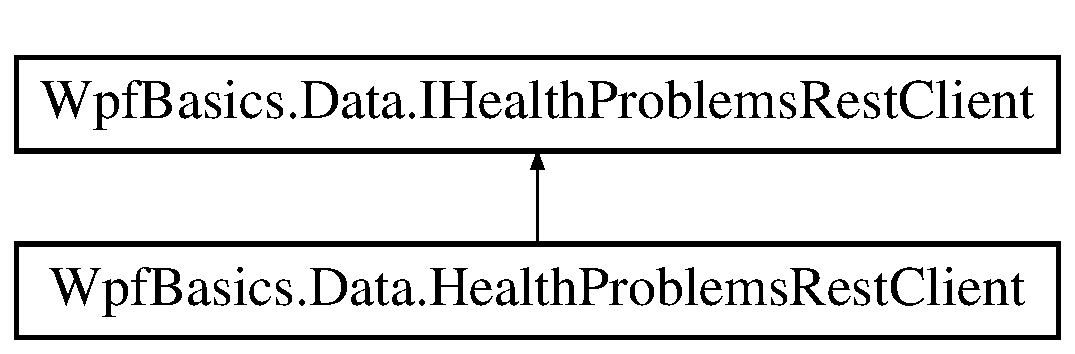
\includegraphics[height=2.000000cm]{class_wpf_basics_1_1_data_1_1_health_problems_rest_client}
\end{center}
\end{figure}
\subsection*{Metody publiczne}
\begin{DoxyCompactItemize}
\item 
string \hyperlink{class_wpf_basics_1_1_data_1_1_health_problems_rest_client_ad8ba9319a858e6933c3ef860ab932cad}{Get\+Health\+Problems\+Json} ()
\end{DoxyCompactItemize}


\subsection{Opis szczegółowy}
Klasa Health\+Problem\+Rest\+Client, utworzenie Resta, połączenie z serwerem Javy. 

\href{http://restsharp.org/}{\tt http\+://restsharp.\+org/} 

\subsection{Dokumentacja funkcji składowych}
\mbox{\Hypertarget{class_wpf_basics_1_1_data_1_1_health_problems_rest_client_ad8ba9319a858e6933c3ef860ab932cad}\label{class_wpf_basics_1_1_data_1_1_health_problems_rest_client_ad8ba9319a858e6933c3ef860ab932cad}} 
\index{Wpf\+Basics\+::\+Data\+::\+Health\+Problems\+Rest\+Client@{Wpf\+Basics\+::\+Data\+::\+Health\+Problems\+Rest\+Client}!Get\+Health\+Problems\+Json@{Get\+Health\+Problems\+Json}}
\index{Get\+Health\+Problems\+Json@{Get\+Health\+Problems\+Json}!Wpf\+Basics\+::\+Data\+::\+Health\+Problems\+Rest\+Client@{Wpf\+Basics\+::\+Data\+::\+Health\+Problems\+Rest\+Client}}
\subsubsection{\texorpdfstring{Get\+Health\+Problems\+Json()}{GetHealthProblemsJson()}}
{\footnotesize\ttfamily string Wpf\+Basics.\+Data.\+Health\+Problems\+Rest\+Client.\+Get\+Health\+Problems\+Json (\begin{DoxyParamCaption}{ }\end{DoxyParamCaption})}

pobranie J\+S\+ON\textquotesingle{}a $<$ pobranie J\+S\+ON\textquotesingle{}a 

Implementuje \hyperlink{interface_wpf_basics_1_1_data_1_1_i_health_problems_rest_client_a1a7509e5e42db251942980c8a0d648d0}{Wpf\+Basics.\+Data.\+I\+Health\+Problems\+Rest\+Client}.



Dokumentacja dla tej klasy została wygenerowana z pliku\+:\begin{DoxyCompactItemize}
\item 
C\+:/\+Users/\+Maria/\+Desktop/\+Suplement\+Selector\+C/Health\+Problems\+Rest\+Client.\+cs\end{DoxyCompactItemize}

\hypertarget{interface_wpf_basics_1_1_data_1_1_i_health_problems_rest_client}{}\section{Dokumentacja interfejsu Wpf\+Basics.\+Data.\+I\+Health\+Problems\+Rest\+Client}
\label{interface_wpf_basics_1_1_data_1_1_i_health_problems_rest_client}\index{Wpf\+Basics.\+Data.\+I\+Health\+Problems\+Rest\+Client@{Wpf\+Basics.\+Data.\+I\+Health\+Problems\+Rest\+Client}}


Klasa I\+Health\+Problem\+Rest\+Client, Interfejs utworzony na potrzeby testów jednostkowych.  


Diagram dziedziczenia dla Wpf\+Basics.\+Data.\+I\+Health\+Problems\+Rest\+Client\begin{figure}[H]
\begin{center}
\leavevmode
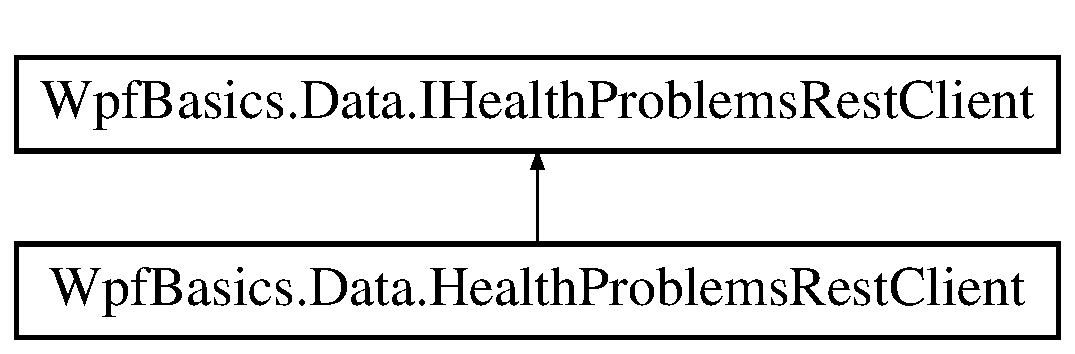
\includegraphics[height=2.000000cm]{interface_wpf_basics_1_1_data_1_1_i_health_problems_rest_client}
\end{center}
\end{figure}
\subsection*{Metody publiczne}
\begin{DoxyCompactItemize}
\item 
string \hyperlink{interface_wpf_basics_1_1_data_1_1_i_health_problems_rest_client_a1a7509e5e42db251942980c8a0d648d0}{Get\+Health\+Problems\+Json} ()
\end{DoxyCompactItemize}


\subsection{Opis szczegółowy}
Klasa I\+Health\+Problem\+Rest\+Client, Interfejs utworzony na potrzeby testów jednostkowych. 

, bez Interfejsu nie da się utworzyć Mocka potrzebnego do testów jednostkowych 

\subsection{Dokumentacja funkcji składowych}
\mbox{\Hypertarget{interface_wpf_basics_1_1_data_1_1_i_health_problems_rest_client_a1a7509e5e42db251942980c8a0d648d0}\label{interface_wpf_basics_1_1_data_1_1_i_health_problems_rest_client_a1a7509e5e42db251942980c8a0d648d0}} 
\index{Wpf\+Basics\+::\+Data\+::\+I\+Health\+Problems\+Rest\+Client@{Wpf\+Basics\+::\+Data\+::\+I\+Health\+Problems\+Rest\+Client}!Get\+Health\+Problems\+Json@{Get\+Health\+Problems\+Json}}
\index{Get\+Health\+Problems\+Json@{Get\+Health\+Problems\+Json}!Wpf\+Basics\+::\+Data\+::\+I\+Health\+Problems\+Rest\+Client@{Wpf\+Basics\+::\+Data\+::\+I\+Health\+Problems\+Rest\+Client}}
\subsubsection{\texorpdfstring{Get\+Health\+Problems\+Json()}{GetHealthProblemsJson()}}
{\footnotesize\ttfamily string Wpf\+Basics.\+Data.\+I\+Health\+Problems\+Rest\+Client.\+Get\+Health\+Problems\+Json (\begin{DoxyParamCaption}{ }\end{DoxyParamCaption})}

pobranie J\+S\+ON\textquotesingle{}a 

Implementowany w \hyperlink{class_wpf_basics_1_1_data_1_1_health_problems_rest_client_ad8ba9319a858e6933c3ef860ab932cad}{Wpf\+Basics.\+Data.\+Health\+Problems\+Rest\+Client}.



Dokumentacja dla tego interfejsu została wygenerowana z pliku\+:\begin{DoxyCompactItemize}
\item 
C\+:/\+Users/\+Maria/\+Desktop/\+Suplement\+Selector\+C/I\+Health\+Problems\+Rest\+Client.\+cs\end{DoxyCompactItemize}

\hypertarget{class_wpf_basics_1_1_main_window}{}\section{Dokumentacja klasy Wpf\+Basics.\+Main\+Window}
\label{class_wpf_basics_1_1_main_window}\index{Wpf\+Basics.\+Main\+Window@{Wpf\+Basics.\+Main\+Window}}


Logika interakcji dla klasy Main\+Window.\+xaml  


Diagram dziedziczenia dla Wpf\+Basics.\+Main\+Window\begin{figure}[H]
\begin{center}
\leavevmode
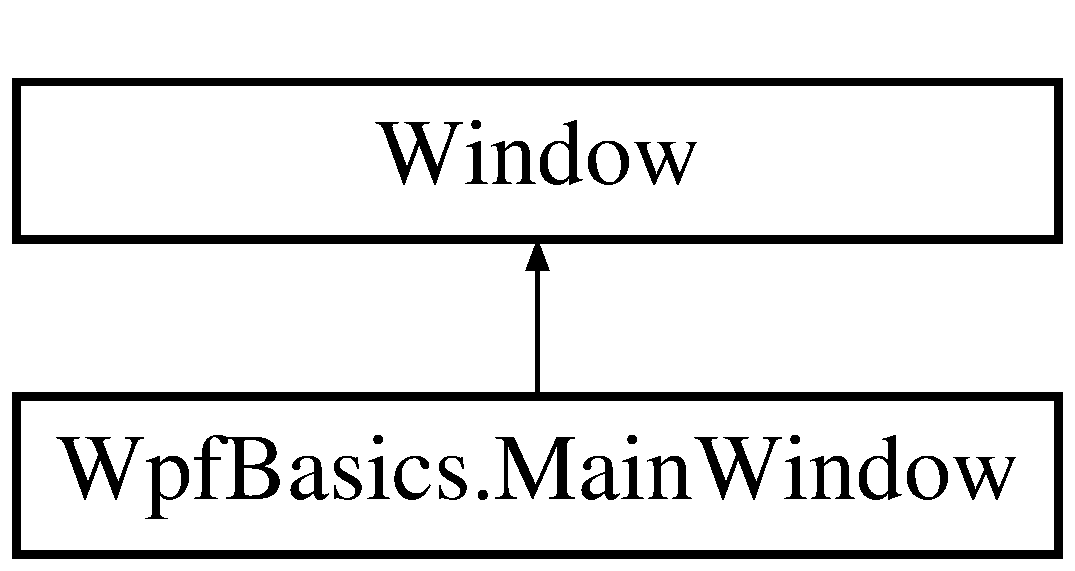
\includegraphics[height=2.000000cm]{class_wpf_basics_1_1_main_window}
\end{center}
\end{figure}


\subsection{Opis szczegółowy}
Logika interakcji dla klasy Main\+Window.\+xaml 

Klasa \hyperlink{class_wpf_basics_1_1_main_window}{Main\+Window}, obsługa zdarzeń

ustawienie obiektu dla Bindingu, utworzenie data\+Loader, metoda przekierowująca na stronę internetowy 

Dokumentacja dla tej klasy została wygenerowana z pliku\+:\begin{DoxyCompactItemize}
\item 
C\+:/\+Users/\+Maria/\+Desktop/\+Suplement\+Selector\+C/Main\+Window.\+xaml.\+cs\end{DoxyCompactItemize}

\hypertarget{class_wpf_basics_1_1_data_1_1_selected_item}{}\section{Dokumentacja klasy Wpf\+Basics.\+Data.\+Selected\+Item}
\label{class_wpf_basics_1_1_data_1_1_selected_item}\index{Wpf\+Basics.\+Data.\+Selected\+Item@{Wpf\+Basics.\+Data.\+Selected\+Item}}


Klasa \hyperlink{class_wpf_basics_1_1_data_1_1_selected_item}{Selected\+Item}, obsługa zdarzeń  


Diagram dziedziczenia dla Wpf\+Basics.\+Data.\+Selected\+Item\begin{figure}[H]
\begin{center}
\leavevmode
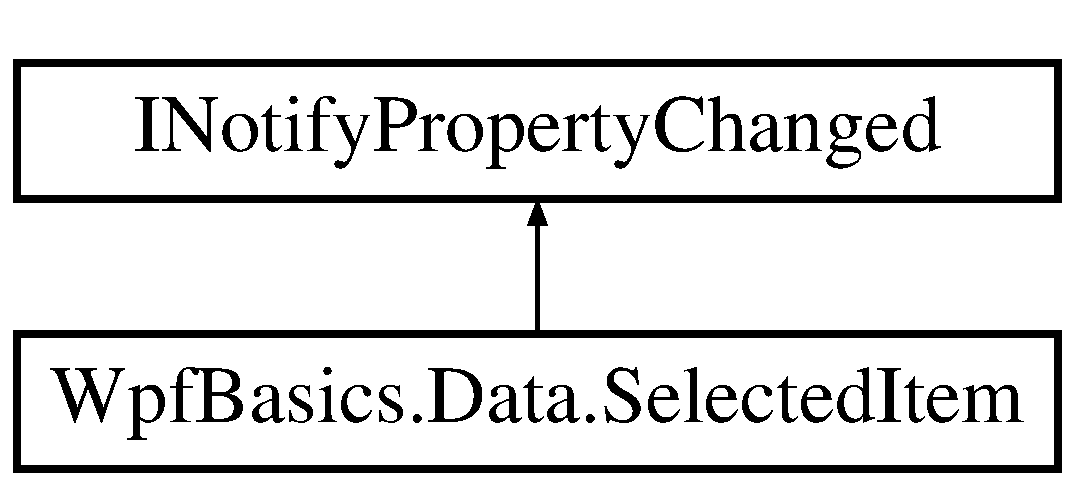
\includegraphics[height=2.000000cm]{class_wpf_basics_1_1_data_1_1_selected_item}
\end{center}
\end{figure}
\subsection*{Właściwości}
\begin{DoxyCompactItemize}
\item 
\hyperlink{class_wpf_basics_1_1_data_1_1_health_problem}{Health\+Problem} \hyperlink{class_wpf_basics_1_1_data_1_1_selected_item_a8d407f9cb4b499f83cb925087262d76a}{Selected\+Health\+Problem}\hspace{0.3cm}{\ttfamily  \mbox{[}get, set\mbox{]}}
\item 
\hyperlink{class_wpf_basics_1_1_data_1_1_suplement}{Suplement} \hyperlink{class_wpf_basics_1_1_data_1_1_selected_item_ab38632718367f7402e49c68bf020913d}{Selected\+Suplement}\hspace{0.3cm}{\ttfamily  \mbox{[}get, set\mbox{]}}
\item 
List$<$ \hyperlink{class_wpf_basics_1_1_data_1_1_health_problem}{Health\+Problem} $>$ \hyperlink{class_wpf_basics_1_1_data_1_1_selected_item_ad36fd63380243a4f18f461fecf26ba16}{All\+Health\+Problems}\hspace{0.3cm}{\ttfamily  \mbox{[}get, set\mbox{]}}
\end{DoxyCompactItemize}
\subsection*{Zdarzenia}
\begin{DoxyCompactItemize}
\item 
\mbox{\Hypertarget{class_wpf_basics_1_1_data_1_1_selected_item_a9acae308d6d33dacb6a7316658f3e0c6}\label{class_wpf_basics_1_1_data_1_1_selected_item_a9acae308d6d33dacb6a7316658f3e0c6}} 
Property\+Changed\+Event\+Handler {\bfseries Property\+Changed}
\end{DoxyCompactItemize}


\subsection{Opis szczegółowy}
Klasa \hyperlink{class_wpf_basics_1_1_data_1_1_selected_item}{Selected\+Item}, obsługa zdarzeń 

Fody\+Weavers notifypropertychanged 

\subsection{Dokumentacja właściwości}
\mbox{\Hypertarget{class_wpf_basics_1_1_data_1_1_selected_item_ad36fd63380243a4f18f461fecf26ba16}\label{class_wpf_basics_1_1_data_1_1_selected_item_ad36fd63380243a4f18f461fecf26ba16}} 
\index{Wpf\+Basics\+::\+Data\+::\+Selected\+Item@{Wpf\+Basics\+::\+Data\+::\+Selected\+Item}!All\+Health\+Problems@{All\+Health\+Problems}}
\index{All\+Health\+Problems@{All\+Health\+Problems}!Wpf\+Basics\+::\+Data\+::\+Selected\+Item@{Wpf\+Basics\+::\+Data\+::\+Selected\+Item}}
\subsubsection{\texorpdfstring{All\+Health\+Problems}{AllHealthProblems}}
{\footnotesize\ttfamily List$<$\hyperlink{class_wpf_basics_1_1_data_1_1_health_problem}{Health\+Problem}$>$ Wpf\+Basics.\+Data.\+Selected\+Item.\+All\+Health\+Problems\hspace{0.3cm}{\ttfamily [get]}, {\ttfamily [set]}}

$<$ pobieranie i ustawianie wartości listy all \mbox{\Hypertarget{class_wpf_basics_1_1_data_1_1_selected_item_a8d407f9cb4b499f83cb925087262d76a}\label{class_wpf_basics_1_1_data_1_1_selected_item_a8d407f9cb4b499f83cb925087262d76a}} 
\index{Wpf\+Basics\+::\+Data\+::\+Selected\+Item@{Wpf\+Basics\+::\+Data\+::\+Selected\+Item}!Selected\+Health\+Problem@{Selected\+Health\+Problem}}
\index{Selected\+Health\+Problem@{Selected\+Health\+Problem}!Wpf\+Basics\+::\+Data\+::\+Selected\+Item@{Wpf\+Basics\+::\+Data\+::\+Selected\+Item}}
\subsubsection{\texorpdfstring{Selected\+Health\+Problem}{SelectedHealthProblem}}
{\footnotesize\ttfamily \hyperlink{class_wpf_basics_1_1_data_1_1_health_problem}{Health\+Problem} Wpf\+Basics.\+Data.\+Selected\+Item.\+Selected\+Health\+Problem\hspace{0.3cm}{\ttfamily [get]}, {\ttfamily [set]}}

$<$ pobieranie i ustawianie wartości wybranego problemu zdrowotnego \mbox{\Hypertarget{class_wpf_basics_1_1_data_1_1_selected_item_ab38632718367f7402e49c68bf020913d}\label{class_wpf_basics_1_1_data_1_1_selected_item_ab38632718367f7402e49c68bf020913d}} 
\index{Wpf\+Basics\+::\+Data\+::\+Selected\+Item@{Wpf\+Basics\+::\+Data\+::\+Selected\+Item}!Selected\+Suplement@{Selected\+Suplement}}
\index{Selected\+Suplement@{Selected\+Suplement}!Wpf\+Basics\+::\+Data\+::\+Selected\+Item@{Wpf\+Basics\+::\+Data\+::\+Selected\+Item}}
\subsubsection{\texorpdfstring{Selected\+Suplement}{SelectedSuplement}}
{\footnotesize\ttfamily \hyperlink{class_wpf_basics_1_1_data_1_1_suplement}{Suplement} Wpf\+Basics.\+Data.\+Selected\+Item.\+Selected\+Suplement\hspace{0.3cm}{\ttfamily [get]}, {\ttfamily [set]}}

$<$ pobieranie i ustawianie wartości wybranego suplementu 

Dokumentacja dla tej klasy została wygenerowana z pliku\+:\begin{DoxyCompactItemize}
\item 
C\+:/\+Users/\+Maria/\+Desktop/\+Suplement\+Selector\+C/Selected\+Item.\+cs\end{DoxyCompactItemize}

\hypertarget{class_wpf_basics_1_1_data_1_1_suplement}{}\section{Dokumentacja klasy Wpf\+Basics.\+Data.\+Suplement}
\label{class_wpf_basics_1_1_data_1_1_suplement}\index{Wpf\+Basics.\+Data.\+Suplement@{Wpf\+Basics.\+Data.\+Suplement}}


Klasa \hyperlink{class_wpf_basics_1_1_data_1_1_suplement}{Suplement}, deklaracja składowych.  


Diagram dziedziczenia dla Wpf\+Basics.\+Data.\+Suplement\begin{figure}[H]
\begin{center}
\leavevmode
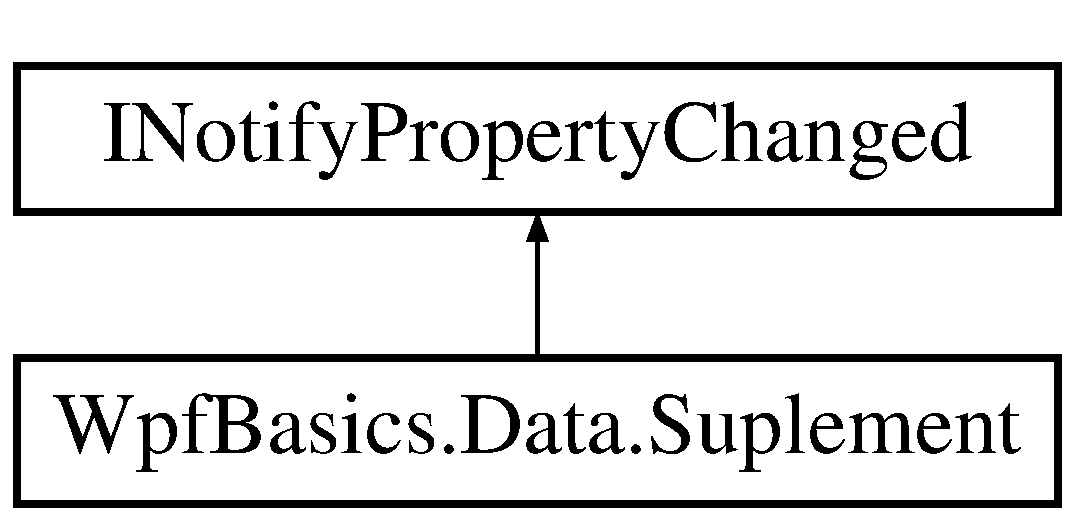
\includegraphics[height=2.000000cm]{class_wpf_basics_1_1_data_1_1_suplement}
\end{center}
\end{figure}
\subsection*{Metody publiczne}
\begin{DoxyCompactItemize}
\item 
override string \hyperlink{class_wpf_basics_1_1_data_1_1_suplement_a1c5a542a7eb2698f1f6cf1d2ea6faa9f}{To\+String} ()
\end{DoxyCompactItemize}
\subsection*{Właściwości}
\begin{DoxyCompactItemize}
\item 
String \hyperlink{class_wpf_basics_1_1_data_1_1_suplement_aa4cc2e887ff276efe8be1cdb94a4a520}{Name}\hspace{0.3cm}{\ttfamily  \mbox{[}get, set\mbox{]}}
\item 
String \hyperlink{class_wpf_basics_1_1_data_1_1_suplement_a020da06c09bf65ffcd1de13550426708}{Chosen\+Suplement}\hspace{0.3cm}{\ttfamily  \mbox{[}get, set\mbox{]}}
\item 
String \hyperlink{class_wpf_basics_1_1_data_1_1_suplement_a5a13a37cdb3c962afa0142ca16056455}{Suplement\+Description}\hspace{0.3cm}{\ttfamily  \mbox{[}get, set\mbox{]}}
\item 
String \hyperlink{class_wpf_basics_1_1_data_1_1_suplement_a94c12d6a1c7db2febb83883f48b259b9}{How\+To}\hspace{0.3cm}{\ttfamily  \mbox{[}get, set\mbox{]}}
\item 
String \hyperlink{class_wpf_basics_1_1_data_1_1_suplement_ada9c156066a12e264b92d6f3ffd3a3f6}{Link\+Url}\hspace{0.3cm}{\ttfamily  \mbox{[}get, set\mbox{]}}
\end{DoxyCompactItemize}
\subsection*{Zdarzenia}
\begin{DoxyCompactItemize}
\item 
\mbox{\Hypertarget{class_wpf_basics_1_1_data_1_1_suplement_a3d338f2485c6b68e4348a89996e8483d}\label{class_wpf_basics_1_1_data_1_1_suplement_a3d338f2485c6b68e4348a89996e8483d}} 
Property\+Changed\+Event\+Handler {\bfseries Property\+Changed}
\end{DoxyCompactItemize}


\subsection{Opis szczegółowy}
Klasa \hyperlink{class_wpf_basics_1_1_data_1_1_suplement}{Suplement}, deklaracja składowych. 

gettey i settery

$<$ korzystanie z biblioteki Inotify 

\subsection{Dokumentacja funkcji składowych}
\mbox{\Hypertarget{class_wpf_basics_1_1_data_1_1_suplement_a1c5a542a7eb2698f1f6cf1d2ea6faa9f}\label{class_wpf_basics_1_1_data_1_1_suplement_a1c5a542a7eb2698f1f6cf1d2ea6faa9f}} 
\index{Wpf\+Basics\+::\+Data\+::\+Suplement@{Wpf\+Basics\+::\+Data\+::\+Suplement}!To\+String@{To\+String}}
\index{To\+String@{To\+String}!Wpf\+Basics\+::\+Data\+::\+Suplement@{Wpf\+Basics\+::\+Data\+::\+Suplement}}
\subsubsection{\texorpdfstring{To\+String()}{ToString()}}
{\footnotesize\ttfamily override string Wpf\+Basics.\+Data.\+Suplement.\+To\+String (\begin{DoxyParamCaption}{ }\end{DoxyParamCaption})}

$<$ zwraca nazwe suplementu 

\subsection{Dokumentacja właściwości}
\mbox{\Hypertarget{class_wpf_basics_1_1_data_1_1_suplement_a020da06c09bf65ffcd1de13550426708}\label{class_wpf_basics_1_1_data_1_1_suplement_a020da06c09bf65ffcd1de13550426708}} 
\index{Wpf\+Basics\+::\+Data\+::\+Suplement@{Wpf\+Basics\+::\+Data\+::\+Suplement}!Chosen\+Suplement@{Chosen\+Suplement}}
\index{Chosen\+Suplement@{Chosen\+Suplement}!Wpf\+Basics\+::\+Data\+::\+Suplement@{Wpf\+Basics\+::\+Data\+::\+Suplement}}
\subsubsection{\texorpdfstring{Chosen\+Suplement}{ChosenSuplement}}
{\footnotesize\ttfamily String Wpf\+Basics.\+Data.\+Suplement.\+Chosen\+Suplement\hspace{0.3cm}{\ttfamily [get]}, {\ttfamily [set]}}

$<$ pobieranie i ustawianie wartości składowej wybrany suplement \mbox{\Hypertarget{class_wpf_basics_1_1_data_1_1_suplement_a94c12d6a1c7db2febb83883f48b259b9}\label{class_wpf_basics_1_1_data_1_1_suplement_a94c12d6a1c7db2febb83883f48b259b9}} 
\index{Wpf\+Basics\+::\+Data\+::\+Suplement@{Wpf\+Basics\+::\+Data\+::\+Suplement}!How\+To@{How\+To}}
\index{How\+To@{How\+To}!Wpf\+Basics\+::\+Data\+::\+Suplement@{Wpf\+Basics\+::\+Data\+::\+Suplement}}
\subsubsection{\texorpdfstring{How\+To}{HowTo}}
{\footnotesize\ttfamily String Wpf\+Basics.\+Data.\+Suplement.\+How\+To\hspace{0.3cm}{\ttfamily [get]}, {\ttfamily [set]}}

$<$ pobieranie i ustawianie wartości składowej w której opisane jest jak stosować, dawkować suplement \mbox{\Hypertarget{class_wpf_basics_1_1_data_1_1_suplement_ada9c156066a12e264b92d6f3ffd3a3f6}\label{class_wpf_basics_1_1_data_1_1_suplement_ada9c156066a12e264b92d6f3ffd3a3f6}} 
\index{Wpf\+Basics\+::\+Data\+::\+Suplement@{Wpf\+Basics\+::\+Data\+::\+Suplement}!Link\+Url@{Link\+Url}}
\index{Link\+Url@{Link\+Url}!Wpf\+Basics\+::\+Data\+::\+Suplement@{Wpf\+Basics\+::\+Data\+::\+Suplement}}
\subsubsection{\texorpdfstring{Link\+Url}{LinkUrl}}
{\footnotesize\ttfamily String Wpf\+Basics.\+Data.\+Suplement.\+Link\+Url\hspace{0.3cm}{\ttfamily [get]}, {\ttfamily [set]}}

$<$ pobieranie i ustawianie wartości składowej z adresem U\+RL do strony internetowej z ofertą \mbox{\Hypertarget{class_wpf_basics_1_1_data_1_1_suplement_aa4cc2e887ff276efe8be1cdb94a4a520}\label{class_wpf_basics_1_1_data_1_1_suplement_aa4cc2e887ff276efe8be1cdb94a4a520}} 
\index{Wpf\+Basics\+::\+Data\+::\+Suplement@{Wpf\+Basics\+::\+Data\+::\+Suplement}!Name@{Name}}
\index{Name@{Name}!Wpf\+Basics\+::\+Data\+::\+Suplement@{Wpf\+Basics\+::\+Data\+::\+Suplement}}
\subsubsection{\texorpdfstring{Name}{Name}}
{\footnotesize\ttfamily String Wpf\+Basics.\+Data.\+Suplement.\+Name\hspace{0.3cm}{\ttfamily [get]}, {\ttfamily [set]}}

$<$ pobieranie i ustawianie wartości składowej nazwa suplementu \mbox{\Hypertarget{class_wpf_basics_1_1_data_1_1_suplement_a5a13a37cdb3c962afa0142ca16056455}\label{class_wpf_basics_1_1_data_1_1_suplement_a5a13a37cdb3c962afa0142ca16056455}} 
\index{Wpf\+Basics\+::\+Data\+::\+Suplement@{Wpf\+Basics\+::\+Data\+::\+Suplement}!Suplement\+Description@{Suplement\+Description}}
\index{Suplement\+Description@{Suplement\+Description}!Wpf\+Basics\+::\+Data\+::\+Suplement@{Wpf\+Basics\+::\+Data\+::\+Suplement}}
\subsubsection{\texorpdfstring{Suplement\+Description}{SuplementDescription}}
{\footnotesize\ttfamily String Wpf\+Basics.\+Data.\+Suplement.\+Suplement\+Description\hspace{0.3cm}{\ttfamily [get]}, {\ttfamily [set]}}

$<$ pobieranie i ustawianie wartości składowej opis suplementu 

Dokumentacja dla tej klasy została wygenerowana z pliku\+:\begin{DoxyCompactItemize}
\item 
C\+:/\+Users/\+Maria/\+Desktop/\+Suplement\+Selector\+C/Health\+Problem.\+cs\end{DoxyCompactItemize}

%--- End generated contents ---

% Index
\backmatter
\newpage
\phantomsection
\clearemptydoublepage
\addcontentsline{toc}{chapter}{Indeks}
\printindex

\end{document}
